\chapter{The LUX-ZEPLIN Experiment}
\label{chap:chap2}

%%-----Chapter quote
\chapterquote{Place holder.}%
{Place holder, xxxx--xxxx}%: Blaa


An accelerated search for WIMP dark matter was made possible by the introduction of dual-phase xenon TPCs, the origins of which date back to the 1970s. The effective use of this technology made the LUX experiment the first sub-zeptobarn detector, placing stronger constraints on dark matter properties than all its predecessors. The next generation LUX-ZEPLIN (LZ) dark matter experiment, located in the Davis Cavern of the Sanford Underground Research Facility (Lead, South Dakota), 4,850 feet under the ground, aims to build on this success in reaching ever-so sensitive WIMP-nucleon cross-sections. This section will introduce the concept of using xenon TPCs for direct detection dark matter searches; detailing the particle interactions, the detection mechanisms and providing an overview of the LZ detector.


%%------------------------------$$
\section{Dual-Phase Xenon TPCs}
\label{sec:dualphaseTPC}

The introduction of dual-phase TPC technology into the domain of direct detection over the past decade has dramatically improved the pace at which the sensitivity to WIMP dark matter has progressed. Dating back to the 1970s \cite{tpc_technology}, TPC technology has made possible the use of liquid and gaseous xenon as a scintillation media to detect particle interactions, leading to ever-more stringent limits on SI and SD WIMP-nucleon cross-sections across a wide range of WIMP masses. The two main variables that strongly impact the sensitivity to WIMPs are the background rates as observed in the WIMP region of interest (ROI) and the amount of xenon held within the TPC.

In comparison to other noble elements, xenon offers several advantages. The large atomic number of xenon ($A=131$), allows for a high sensitivity to SI-WIMP interactions due to the coherent scattering enhancement ($\propto A^2$) as given by equation (\ref{eq:si_rate}). At relatively low energy thresholds (e.g. $\sim17$ keV for 100 GeV/c$^2$ WIMPs), xenon is the most sensitive noble element of these targets. A comparison of the SI differential event rate for a collection of targets is shown in figure (\ref{fig:nuclear_recoil_rates}). The large atomic number also gives xenon excellent self-shielding properties in slowing down and stopping backgrounds originating from instrumental surfaces within a relatively short distance. The natural abundance of odd-neutron isotopes found in sourced xenon also provides a sensitivity for SD interactions. A major strength for these detectors is the possibility of precise fiducialisation of the xenon volume due to the 3D position reconstruction, allowing for an effective way to reject backgrounds from radiogenic walls and surfaces of the TPC. Furthermore, interaction lengths for gammas and neutrons in LXe are $\sim10 \; \MathText{cm}$ and $\sim15 \; \MathText{cm}$, respectively; hence identifying and rejecting multiple scatters are of critical importance in reducing backgrounds.
%
\begin{figure}[hb!]
    \begin{center}
        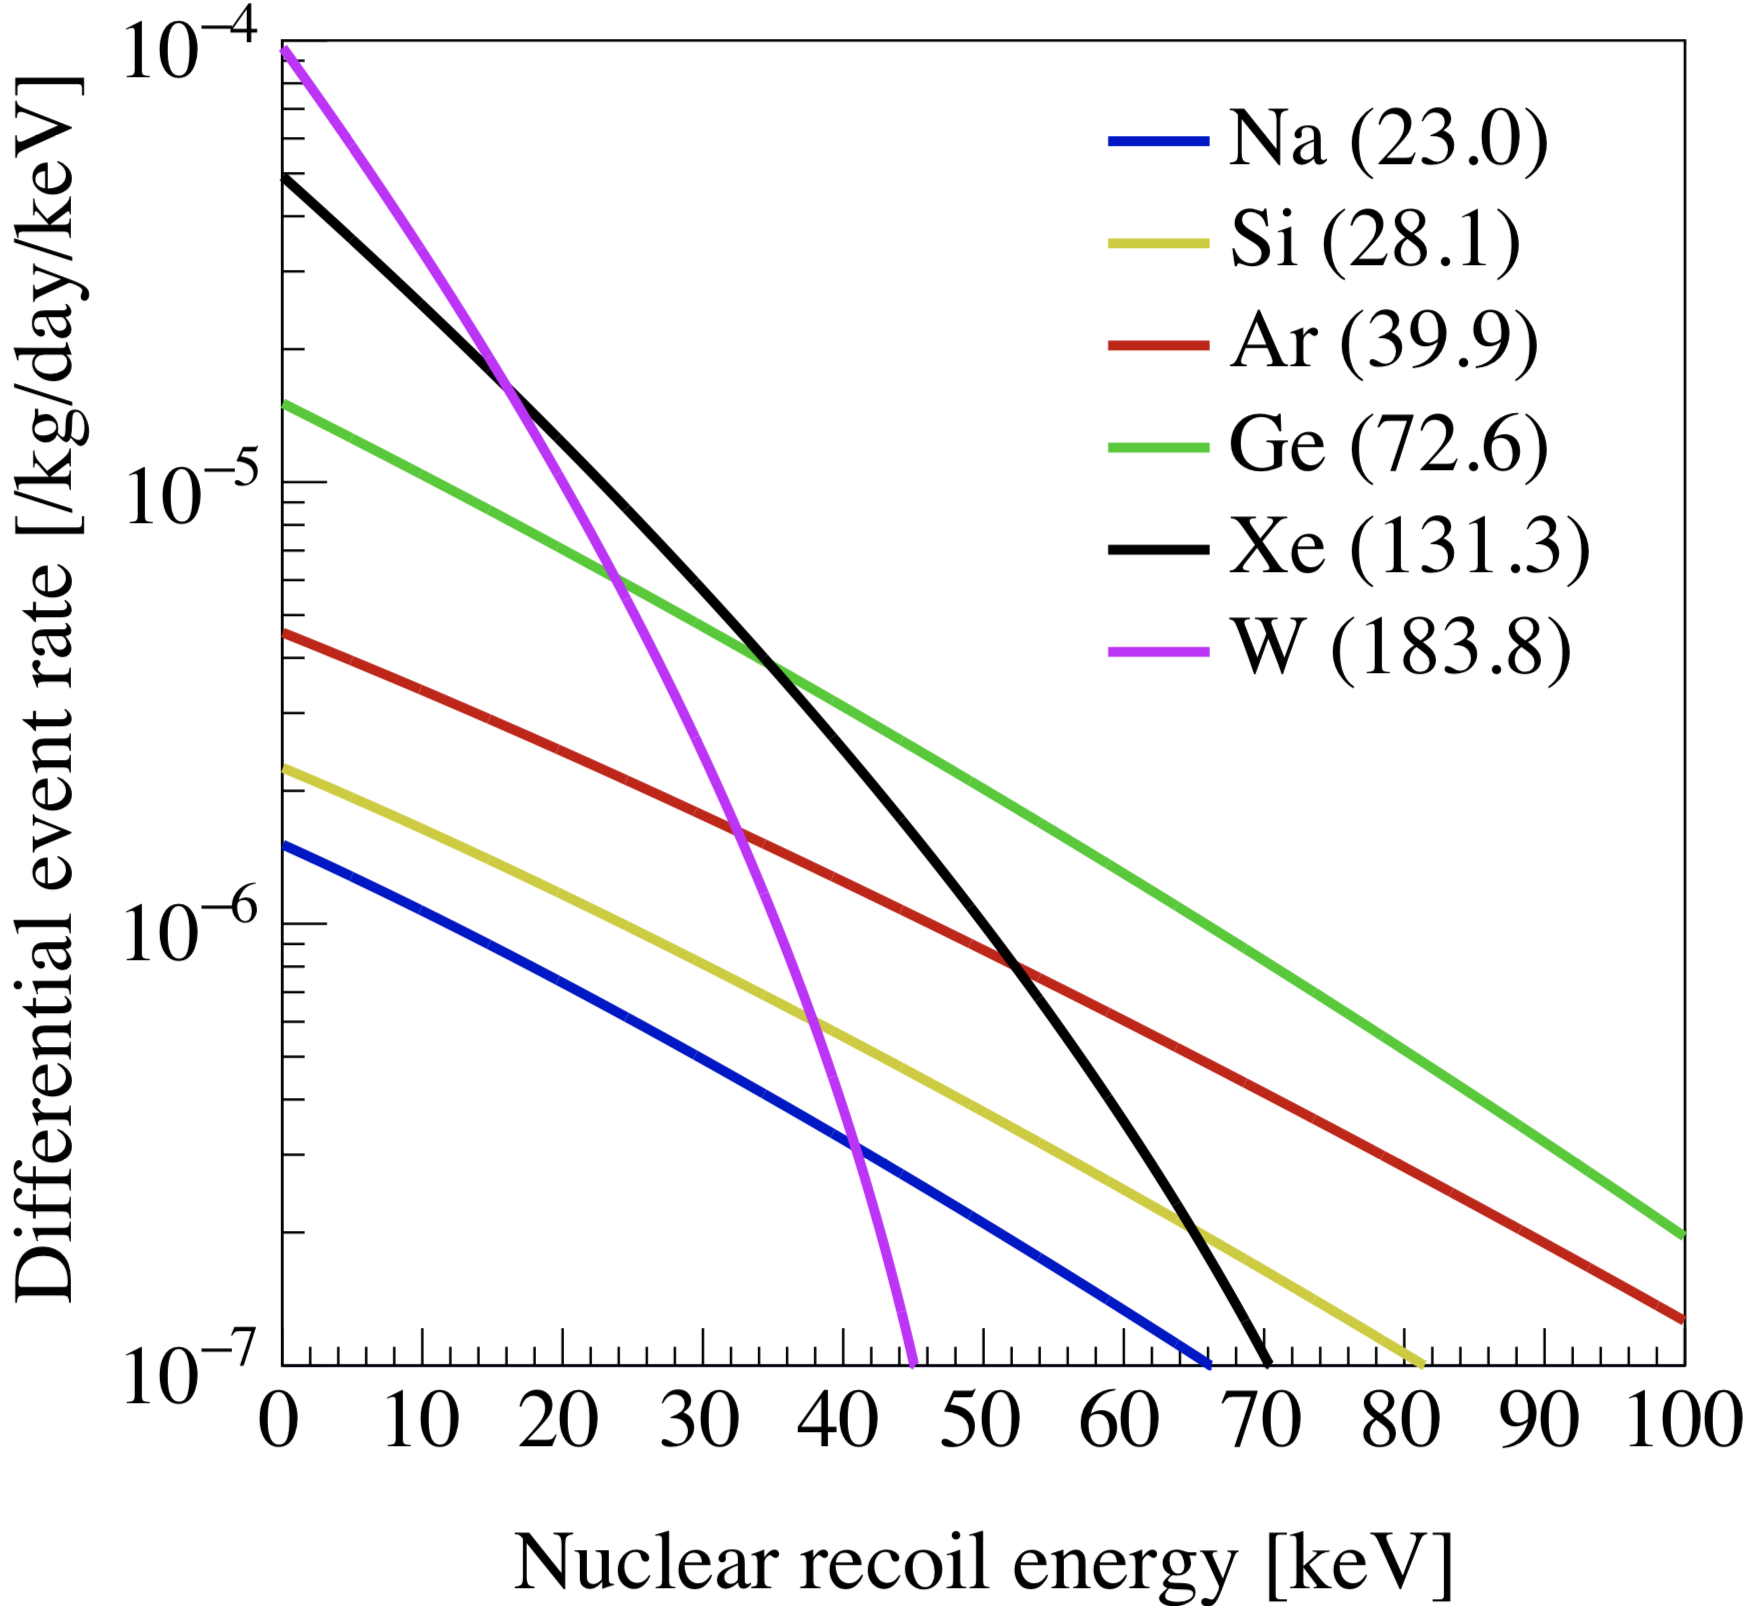
\includegraphics[scale=0.30]{Chapter_2/Figures/SI_nuclear_recoil_rates.png}
        \caption[Comparison of differential event rates of a $100 \MathText{GeV/c}^{2}$ WIMP interaction with several different target material, for an assumed cross-section of $\sigma^{SI}_{N} = 1 \MathText{zb}$]%
        {Comparison of differential event rates of a $100 \MathText{ GeV/c}^{2}$ WIMP interaction with several different target material with an assumed WIMP-nucleon cross-section of $\sigma^{SI}_{N} = 1 \MathText{ zb}$. The averaged atomic mass of each target element at natural abundance is indicated next to its symbol in the legend.}
        \label{fig:nuclear_recoil_rates}
        \end{center}
\end{figure}
%

The interactions taking place inside the TPC generate three types of signals, of which two can be read out by detectors alike. The first of these are the scintillation photons that are produced in the LXe volume via a mechanism that allows these photons to propagate through the liquid and be detected by VUV-sensitive PMTs that cover the top and bottom of the TPC. The interaction also produces ionisation electrons that are drifted upwards via a vertical electric field of several $100 \MathText{ V/cm}$. Once they reach the liquid surface, these electrons are extracted and accelerated through the gaseous phase, producing electroluminescence light, that which is detected by the PMTs. The following sections will cover in detail the mechanisms in which these signals are produced and how they lead to a precise 3D position reconstruction and an effective background discrimination. 


%%------------------------------$$
\section{Particle Interactions \& Detection in a Dual-Phase Xenon TPC}
\label{sec:xenonphysics}

Interactions of particles inside a xenon TPC result in electron and nuclear recoils. Majority of the backgrounds originating from radioactive isotopes, such as beta or gamma particles interact mostly via electron recoils, leading to a significant ER rate. Neutral particles, such as neutrons or WIMPs are expected to undergo nuclear recoils. Electron recoils are interactions in which the incoming particle interacts with the orbital electrons of the xenon atoms, whereas nuclear recoils are kinetic interactions off of the atomic nucleus. The recoiling particles in both cases deposit their energy through multiple short-ranged interactions, forming a track in which a cascade of interactions take place. The end result of this cascade converts the initial particle energy into scintillation photons, ionisation electrons and atomic motion (heat), latter of which is undetectable by current TPCs. The following sections will discuss in detail the mechanisms of energy transfer and signal production in such interactions.

\subsection{Primary Energy Transfer}
\label{sec:energy_transfer}

In rare gases, such as xenon and argon, the energy deposited by radiation is expanded into the production of a number of electron-ion pairs ($N_{ion}$), excited atoms ($N_{ex}$) and thermalised free electrons, known as sub-excitation electrons liberated in the ionisation process. The deposited energy $E_{0}$ can be expressed into ionisation, excitation, and sub-excitation electrons by the use of a Platzman equation \cite{Platzman, xenon_physics}:
%
\begin{equation} \label{eq:e_transfer}
    E_{0} = N_{ion}E_{ion} + N_{ex}E_{ex} + N_{ion}\eta
\end{equation} 
%
where $E_{ion}$ and $E_{ex}$ are the mean ionisation and excitation energies, $N_{ion}$ and $N_{ex}$ are the number of ionised and excited atoms, and $\eta$ is the mean kinetic energy of ionised electrons. The energy required to produce a single electron-ion pair can be taken as an averaged value, defined as the W-value, where,
%
\begin{equation} \label{eq:e_transfer}
    W = E_{0}/N_{ion} = E_{ion} + E_{ex}(N_{ex}/N_{ion}) + \eta.
\end{equation} 
%
The average energy loss in ionisation is slightly larger than the ionisation potential or the band gap energy, resulting in the ratio of the W-value to that of ionisation potential or band gap to be 1.6-1.7 \cite{PhysRevA.48.1313}. In general, the W-value is smaller in the liquid phase, and in LXe, in comparison to liquid argon and neon. As a consequence, the ionisation yield in LXe is the highest of all noble liquids.

Although the above equation is believed to apply for electronic recoils, in the case of nuclear recoils, a large fraction of the deposited energy is spent in nuclear collisions, which do not result in either excitations or ionisations. Hence, an additional term may be considered in equation (\ref{eq:e_transfer}) to account for this loss. The ratio of $N_{ex}/N_{ion}$ has been measured to be $\sim0.2$ for electronic recoils and yields a value of $\sim1$ for nuclear recoils upon fitting to data \cite{xenon_physics, Dahl}. This different in the initial ratio of exciton and electron-ion production is thought to be the underlying principle of discrimination between electron and nuclear recoils in two-phase TPCs. Further discussion on discrimination will follow in section (\ref{subsubsec:recom_disc}).


\subsection{Primary Scintillation (S1)}
\label{subsec:s1}


The primary scintillation light---often referred to as an S1 signal---is produced via a process known as self-trapping, in which an excited xenon atom ($Xe^{\ast}$) forms a molecular dimer ($Xe^{\ast}_{2}$) with a neighbouring atom; the decay of which produces a VUV photon. Upon initial recoil, there are two distinct processes in particular that lead to S1 light production. The first of these are when an incoming particle creates an excited xenon atom, which leads to the creation and decay of an excited xenon dimer molecule \cite{xenon_physics}:
%
\begin{align} \label{eq:exciton_luminescence}
    &p_{i} + Xe \rightarrow Xe^{\ast} + p_{i} \\
    &Xe^{\ast} + Xe \rightarrow Xe^{\ast, v}_{2} \\
    &Xe^{\ast, v}_{2} + Xe \rightarrow Xe^{\ast}_{2} + Xe \\
    &Xe^{\ast}_{2} \rightarrow  Xe +  Xe + \gamma
\end{align}
%
where $p_{i}$ is the incoming particle, representative of any of the primary particle candidates present in such detectors, i.e., electrons, gamma rays, neutrons and so on. The superscript $v$ is used to distinguish vibrationally excited states from purely electronic excitation. The de-excitation of a vibrational state is mostly non-radiative but emission of infrared photons are also possible. The process detailed above is often referred to as \textit{exciton luminescence}.

An alternative process to exciton luminescence is \textit{recombination luminescence}. Although the end result of this process is identical to that of the process above, the initial interaction results in an ionised xenon atom, which undergoes recombination:
%
\begin{align} \label{eq:recombination_luminescence}
    &p_{i} + Xe \rightarrow Xe^{+} + p_{i} + e^{-} \\
    &Xe^{+} + Xe + Xe \rightarrow Xe^{+}_{2} + Xe \\
    &Xe^{+}_{2} + e^{-} \rightarrow Xe^{\ast\ast} + Xe \\
    &Xe^{\ast\ast} + Xe \rightarrow Xe^{\ast} + Xe + (heat) \\
    &Xe^{\ast} + Xe \rightarrow Xe^{\ast, v}_{2} \\
    &Xe^{\ast, v}_{2} + Xe \rightarrow Xe^{\ast}_{2} + Xe \\
    &Xe^{\ast}_{2} \rightarrow  Xe +  Xe + \gamma
\end{align}
%
The emission spectrum of the VUV scintillation photons originating from these two processes are similar as they share a common final stage. In a single event, both of these processes contribute in creating the summed S1 pulse---the collection of the VUV photons originating from an interaction site. However, it's important to note that the rate of recombination luminescence is heavily dependent on the initial energy recoil and more importantly, the electric field applied \cite{Dahl}. Application of an electric field serves as a mechanism to drift away any free electrons from the interaction site, hence suppressing recombination luminescence. 

Although there exists a probability for an optical transition of the excited atoms to undergo a transition to the ground state, the collision rates in liquid xenon often result in the formation of strongly bound two-atomic xenon molecules. These molecules are only bound in their excited states and can exist either in a single state ($^{1}\Sigma^{+}_{u}$) or a triplet state ($^{3}\Sigma^{+}_{u}$), thereafter transitioning to the repulsive ground state ($^{1}\Sigma^{+}_{g}$), where the two molecules separate into two neutral xenon atoms and emit a VUV photon centered at $\sim 178 \; \MathText{nm}$ \cite{FUJII2015293}. Thus, there is no re-absorption of the emitted photon, making xenon highly transparent to its own scintillation light, which is an important feature for a scintillator. The decay time constants of singlet and triplet states are very short, roughly 2.2 ns and 27 ns, respectively \cite{xenon_physics}. But recombination as highlighted under equation (\ref{eq:exciton_luminescence}) is a slow process and can impact the shape of the S1 pulse by adding a non-exponential third component, besides the fast (singlet decay) and the slow (triplet decay) components. The application of an electric field usually serves to reduce this third component by extracting the free electrons.

Furthermore, particle interactions at high energies ($\geq{}\MathText{MeV}$), such as $\alpha$-particles, can lead to the emergence of higher order processes that can decrease the number of primary scintillation photons. At these energies, the particle tracks formed due to high linear energy transfer (LET) increases the density of excited xenon atoms, thereby increasing the probability of interaction between two exited atoms. This process often leads to increase the ionisation rate in the track via a process called \textit{bi-excitonic quenching} \cite{bi_excitonic}:
%
\begin{equation} \label{eq:bi-excitonic_quenching}
    Xe^{\ast} + Xe^{\ast} \rightarrow Xe^{+} + Xe + e^{-}
\end{equation} 
%
A similar process dubbed as \textit{penning ionisation} can also take place if a single excited xenon atom has enough energy to ionise a neutral xenon atom from the ground state:
\cite{Dahl}:
%
\begin{equation} \label{eq:bi-excitonic_quenching}
    Xe^{\ast} + Xe \rightarrow Xe^{+} + Xe + e^{-}
\end{equation} 
%
In such processes, the excited xenon atoms have enough kinetic energy to ionise another atom upon a collision. These processes on average usually leads to the suppression of the summed S1 pulse at higher energy recoils, as the process reduces the probability of exciton luminescence, which often leads to the creation of a VUV photon. Further discussion on the implications of this phenomena will be examined in section (\ref{subsec:light_charge}).

\subsection{Ionisation \& Secondary Scintillation (S1)}
\label{subsec:s2}

The electrons which escape recombination are drifted up by a vertical electric field, effectively removing the electrons from the interaction site. The drift velocity of the electrons depend on the strength of the applied electric field. For liquid xenon, a field strength of $\sim 1 \; \MathText{kV/cm}$ can lead to a $2.25 \; \MathText{mm/\mu{}m}$ drift velocity. After about $10 \; \MathText{kV/cm}$, this dependence no longer holds and the drift velocity saturates at $\sim2.8 \; \MathText{mm/\mu{}m}$ \cite{e_drift}. An accurate understanding of the drift velocity and hence the applied electric field is important in reconstructing the depth (z or the t axis) at which the interaction took place, as this is proportional to the time difference between the S1 signal and the S2 signal---or the time it takes for the electrons to travel to the surface of the liquid.

The ionisation electrons drifting in a TPC will also experience diffusion in all three spacial dimensions. Diffusion taking place across the x-y plane dubbed as transverse diffusion ($D_{T}$) and the z plane, also known as longitudinal diffusion ($D_{L}$). The transverse diffusion usually has no first-order effect on the shape of the summed S2 pulse, whereas despite being an order of magnitude smaller ($D_{L}/D_{T} \simeq 0.1$), the longitudinal diffusion in LXe has a critical effect on the S2 shape because it dictates the photon time of arrival at the photo-detectors. Hence modelling this accurately is crucial for realistic simulations of pulses.

Furthermore, electronegative molecules such as $O_{2}$, $H_{2}O$ and $N_{2}O$ can dramatically decrease the mobility of drifting electrons. These molecules can capture free electrons and form negative ions with extremely low mobility, resulting in drift velocities of a few mm/s at practical electric fields. The probability of a capture by such species depend on the concentration, the reaction rate constant and the path length of the electron as it drifts towards the anode. These species are usually present in sourced xenon and often out-gas from detector material, constantly contaminating the LXe. Hence, the purification of liquefied rare gases to better than ppb level is a critical issue, especially for events at lower energies.

In reaching the liquid surface, the electrons have to overcome a potential barrier to be extracted over into the gas phase. This process is energetically unfavourable and hence an electric field of several kV/cm is usually applied between a grid just below and just above the liquid surface. Once extracted, the electrons are accelerated through the gaseous layer to sufficient energies to excite the gas atoms, thus produce secondary scintillation, also known as electro-luminescence. This process allows very high amplification gains to be achieved, where signals due to a single initial electron to be detected. The mechanism in which secondary scintillation photons are produced is similar to that explained for primary scintillation. A schematic diagram of a toy TPC, highlighting signal generation from an S1 and an S2 signal is depicted in figure (\ref{fig:tpc_diagram}). 
%
\begin{figure}[hb!]
    \begin{center}
        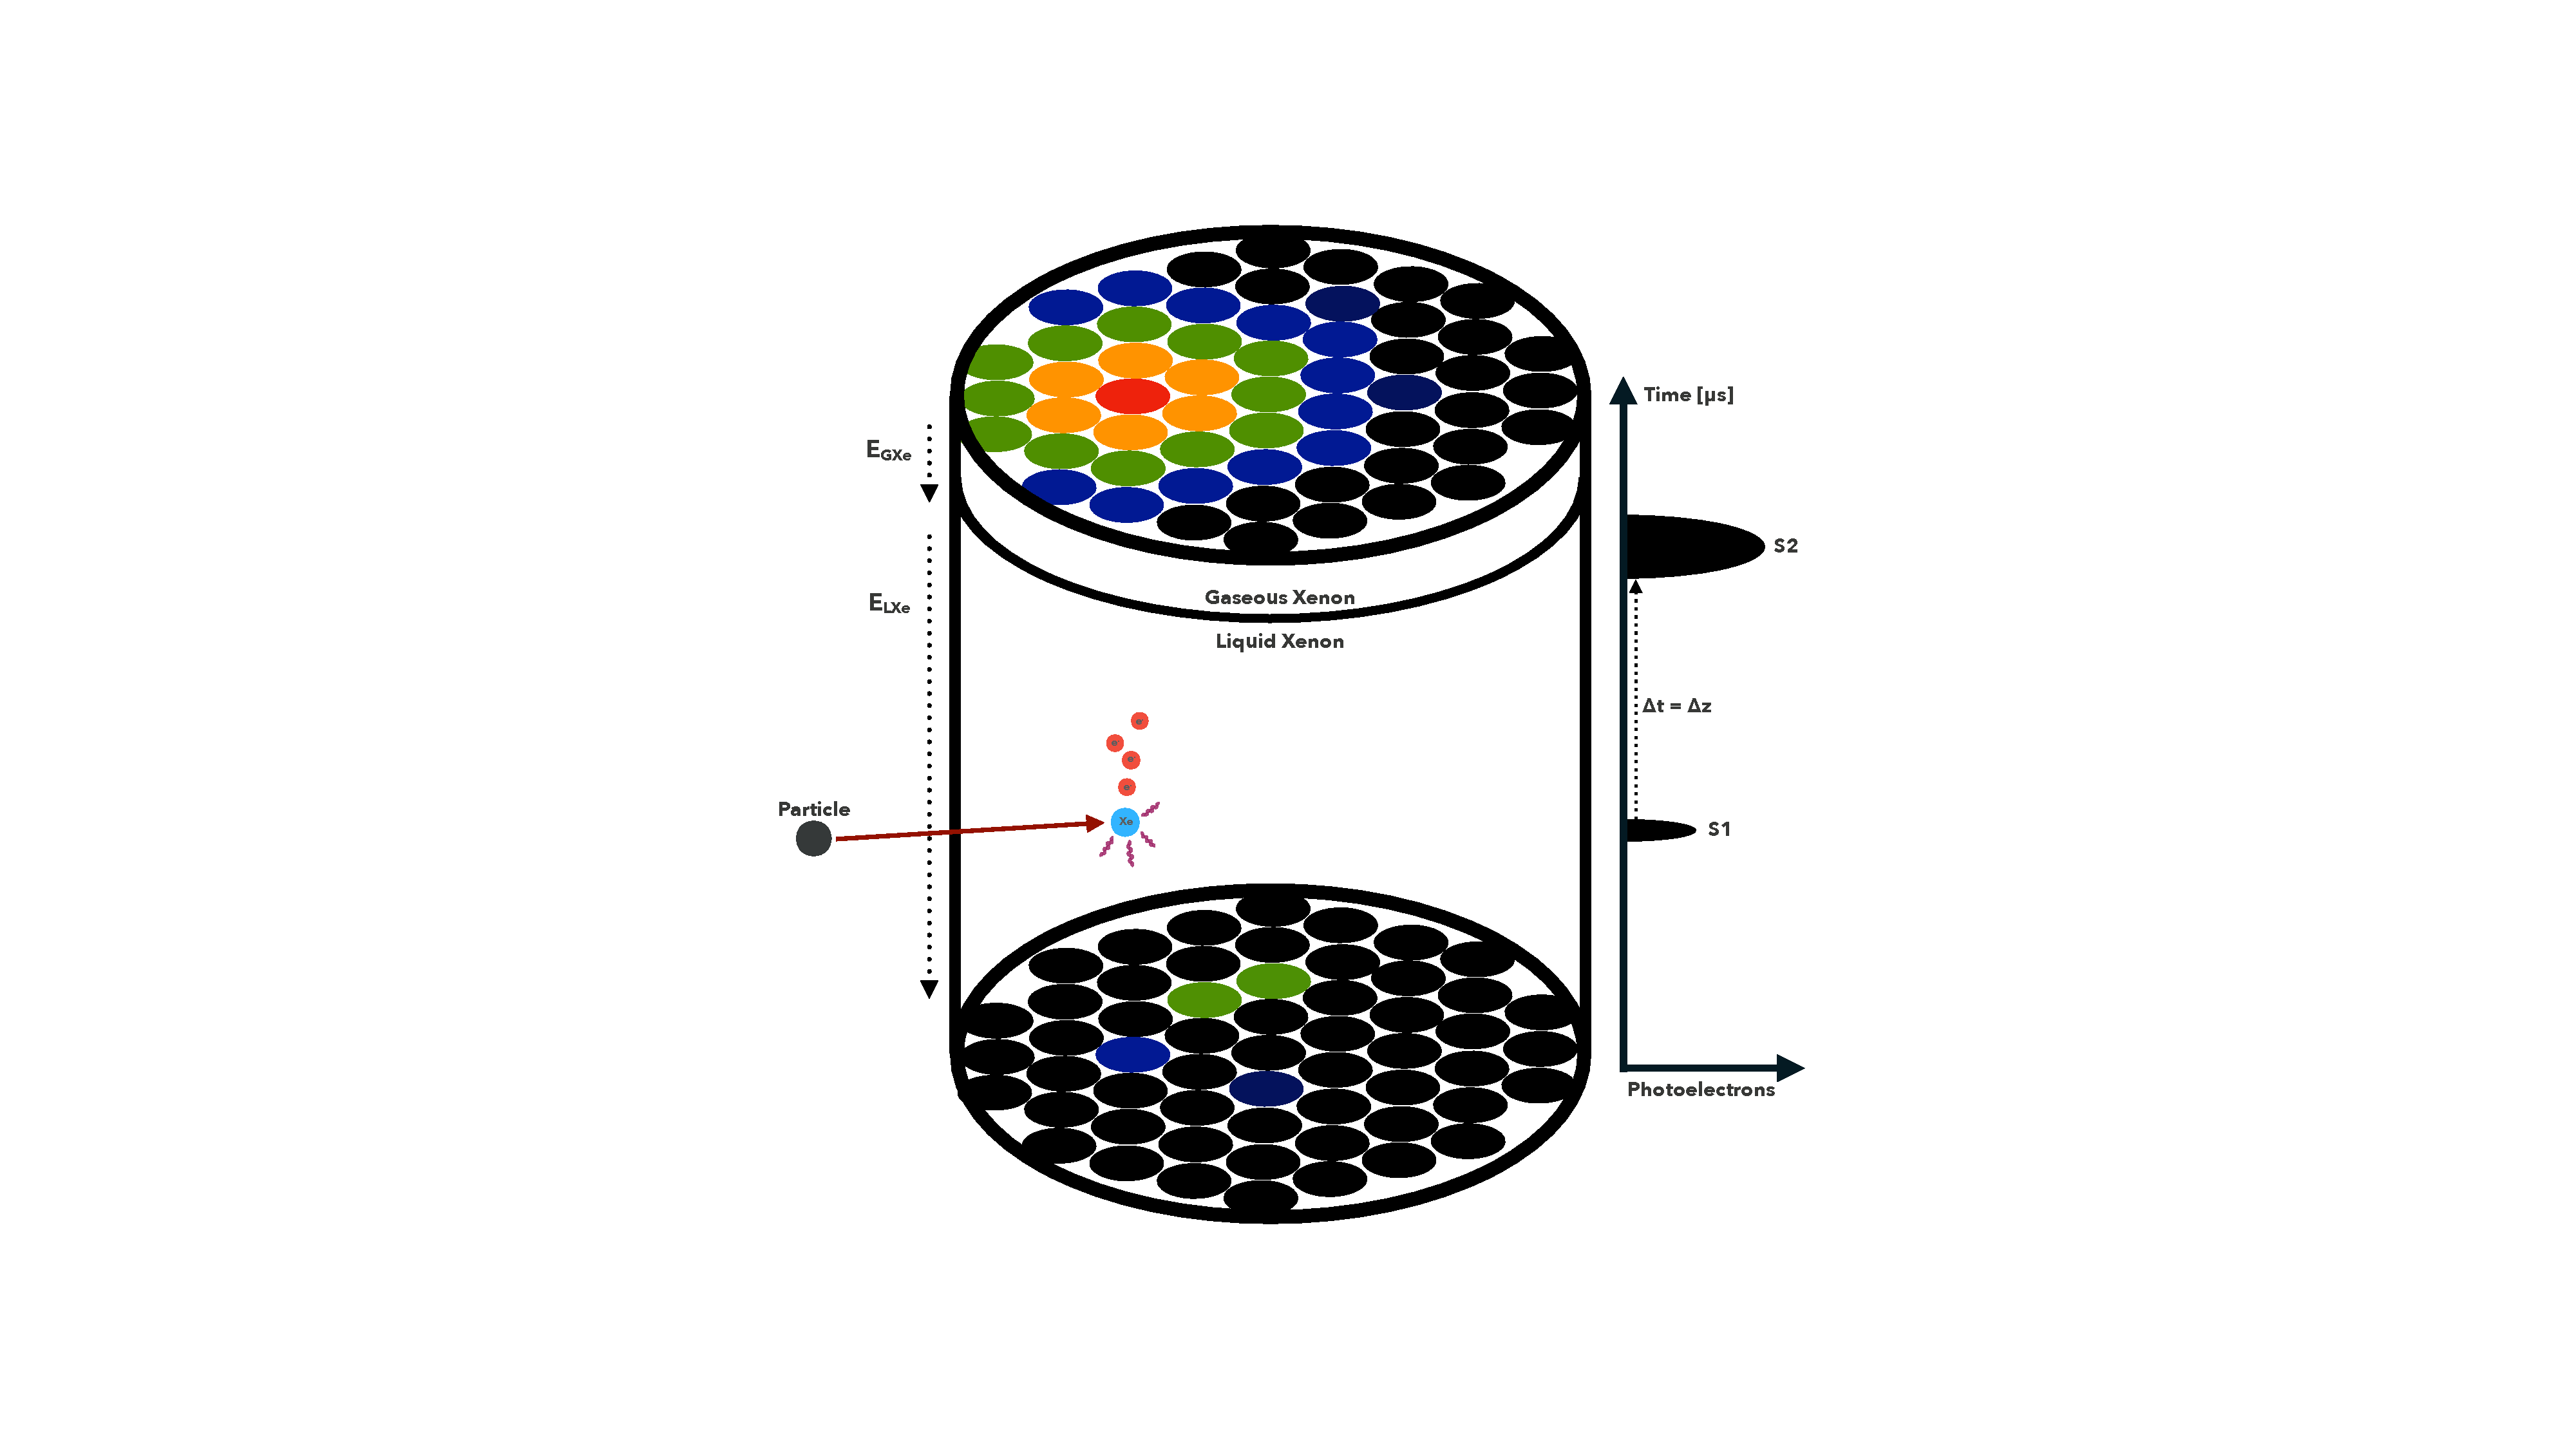
\includegraphics[scale=0.30]{Chapter_2/Figures/TPC_Diagram.pdf}
        \caption[Schematic of a single scatter event inside a dual-phase toy TPC, showing the S1 signal production and the drift of free electrons towards the gas layer]%
        {Schematic of a single scatter event inside a dual-phase toy TPC, showing the S1 signal production and the drift of free electrons towards the gas layer. The top and the bottom of the TPC is covered by PMTs that eventually detect the VUV photons created both in the liquid and in the gas phase. The diagram also depicts how TPCs allows for a 3D position reconstruction; where z is determined by the drift time of electrons and x-y determined by the PMT hit pattern.}
        \label{fig:tpc_diagram}
        \end{center}
\end{figure}
%

\subsection{Energy Reconstruction and Signal Yields}
\label{sec:energy_recon_signal_yields}

Although the underlying principles that go into S1 and S2 production are relatively trivial, the modelling of these processes and correlating the output signal from a detector to a set of initial conditions is less so. Taking into account the above, the number of emitted VUV photons ($n_{\gamma}$) and the escaped electrons ($n_{e}$) in a particle interaction site after recombination can be expressed as,
%
\begin{equation} \label{eq:bi-excitonic_quenching}
    &n_{\gamma} = N_{ex} + rN_{ion} \\
    &n_{e} = (1 - r)N_{ion}
\end{equation}
%
where $N_{ex}$ and $N_{ion}$ are the total number of excited and ionised xenon atoms prior to recombination, respectively, and $r$ is the probability of recombination. In the previous section, it was shown 




\subsubsection{Light \& Charge Yields in Liquid Xenon}
\label{subsubsec:light_charge}




\subsection{Recombination \& Discrimination}
\label{subsubsec:recom_disc}





%%------------------------------$$
\section{The LUX-ZEPLIN Experiment}
\label{sec:lz_detector}



\subsection{TPC \& Skin Detectors}
\label{subsec:tpc_skin}}

\subsection{Cryogenics \& Xenon Handling}
\label{subsec:crypo_xenon}}

\subsection{Outer Detector}
\label{subsec:od}}

\subsection{Outer Detector}
\label{subsec:od}}

\subsection{Calibrations}
\label{subsec:calibrations}}

\subsection{Data Acquisition}
\label{subsec:daq}}




\section{Conclusion}





